\section{Task: Calculate Radar Plot Positions}
\label{sec:task_calc_radar_pos}

This task allows calculation of Radar plot position information based on the defined data sources.

\begin{figure}[H]
  \hspace*{-2.5cm}
    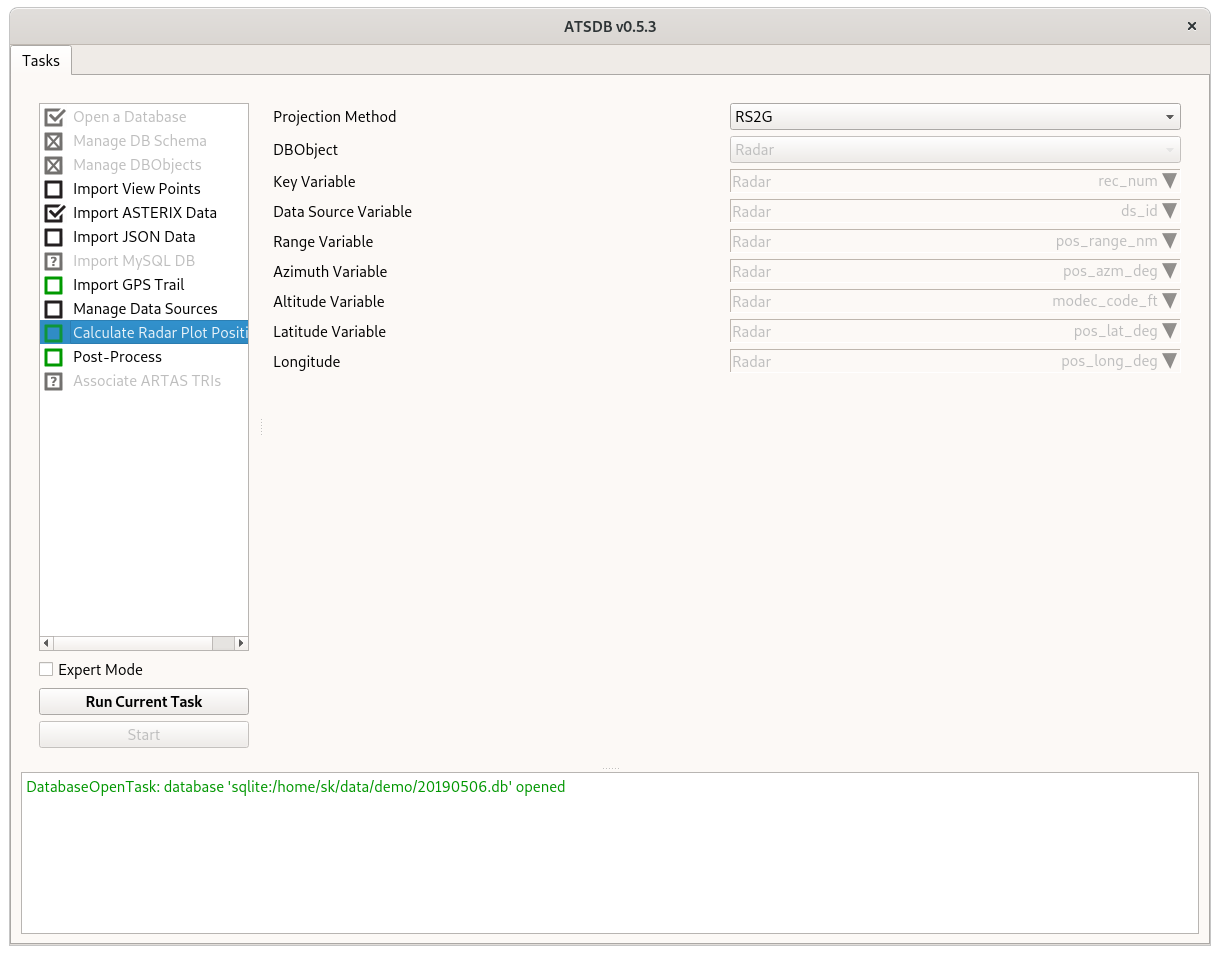
\includegraphics[width=19cm]{../screenshots/task_calc_radar.png}
  \caption{Task: Calculate radar plot positions}
  \label{fig:task_calc_radar}
\end{figure}


Please note that for this step the Radar data source positions have to set in the database (see \nameref{sec:manage_datasources}), otherwise no plot position can be calculated. 

There are two projection methods (radar polar coordinates to WGS-84 coordinates) available. The \textit{RS2G} projection is the currently recommended option.

\paragraph{OGR Projection}

The EPSG code for the projection has to be chosen according to your needs, please refer to \url{http://spatialreference.org/ref/epsg/} for a list of possible codes.

The WGS84 latitude/longitude coordinates are then calculated using the radar positions in the database, the range and the azimuth. Please \textbf{note} that currently there will be offsets in the projected coordinates compared to the e.g. the ARTAS projection. The reason for this is under investigation.

\paragraph{RS2G Projection}

For this projection, no additional attributes must be given. Please \textbf{note} that this projection is based on a common 'radar slant to geodesic transformation', it should be equvalent to the ARTAS projection. A verification is still needed, please contact the author if you would be willing to support this.

\paragraph{Running}

Using the 'Run Current Task' button the task can be performed. During import a status indication will be shown:

\begin{figure}[H]
  \center
    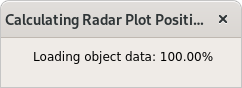
\includegraphics[width=5cm]{../screenshots/task_calc_radar_load.png}
  \caption{Calculate Radar Plot Positions task: Loading}
\end{figure}

\begin{figure}[H]
  \center
    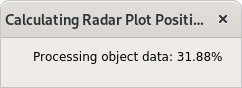
\includegraphics[width=5cm]{../screenshots/task_calc_radar_process.png}
  \caption{Calculate Radar Plot Position task: Processing}
\end{figure}

If there were projection errors in the calculation, the before insertion the user will be asked to confirm. The coordinates with projection errors will of course not be committed to the database, but will be skipped.

\begin{figure}[H]
  \center
    \includegraphics[width=9cm,frame]{../screenshots/task_calc_radar_insert.png}
  \caption{Calculate Radar Plot Position task: Insertion question on errors}
\end{figure}


\begin{figure}[H]
  \center
    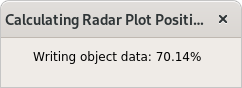
\includegraphics[width=5cm]{../screenshots/task_calc_radar_write.png}
  \caption{Calculate Radar Plot Position task: Writing}
\end{figure}

\begin{figure}[H]
  \center
    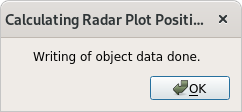
\includegraphics[width=5cm]{../screenshots/task_calc_radar_done.png}
  \caption{Calculate Radar Plot Position task: Done}
\end{figure}

After running this task once (per database), the radar plots also have a set latitude/longitude. As stated, a post-processing step is recommended after executing this task. \\

Please \textbf{note} that this task can be re-run with different projections if wanted.

Please \textbf{note} that no additional Radar plot information is changed, only the latitude/longitude variables are updated. 
